\section*{Глава 2\\Основные соотношения механики упругих анизотропных тел}
\addcontentsline{toc}{section}{Глава 2. Основные соотношения механики упругих анизотропных тел}
\setcounter{section}{2}
\setcounter{subsection}{0}
\setcounter{equation}{0}

\subsection{Тензор упругих постоянных}

	В одномерном случае при не слишком больших деформациях напряжение будет линейно зависеть от деформаций.
	В случае трёх пространственных переменных эта связь в самом общем случае будет иметь вид\cite{resler}:
\begin{align}
	\label{rheology_equation}
	\sigma_{ij} &= C_{ijkl}\varepsilon_{kl},
\end{align}
	где $\sigma_{ij}$ -- тензор напряжений, $\varepsilon_{kl}$ -- тензор деформаций, $C_{ijkl}$ -- тензор упругих постоянных. 
	Это уравнение, по сути, реологическое соотношение из \eqref{initial_equations}.
	
	В общем случае $C_{ijkl}$ имеет $3^{4} = 81$ компоненты. Однако, тензор деформаций симметричен по определению и имеет шесть независимых компонент.
	Тензор напряжений также симметричен, поскольку при его определении мы не учитываем изгибающие моменты\cite{resler}. 
	Во всяком случае, существенно то, что тензор напряжений может быть приведён в симметричному виду\cite{landau_lifshits}.
	
	Таким образом количество независимых компонент тензора упругих постоянных сокращается до $6^{2} = 36$.
	Далее, в упругом случае, тензор упругих постоянных обладает дополнительной симметрией, за счёт потенциальности упругого деформирования. Обозначим $w$ -- потенциал уругости, тогда по определению: $dw = \sigma_{ij} d\varepsilon_{ij}$.
	Учитывая, что: 
\begin{align}
	C_{ijkl} &= \frac{\partial{\sigma_{ij}}}{\partial{\varepsilon_{kl}}},
\end{align}
	имеем:
\begin{align}
	C_{ijkl} &= \frac{\partial^{2}{w}}{\partial{\varepsilon_{ij}\varepsilon_{kl}}}.
\end{align}
	Последовательность вычисления производных в данном случае не имеет значения, поэтому $C_{ijkl} = C_{klij}$ и тензор упругих постоянных имеет 21 независимую компоненту.
	Выражение \eqref{rheology_equation} с симметричной матрицей упругих постоянных \eqref{anisotropic_tensor} теперь удобно записать в виде:
\begin{align}
\left( \begin{array}{cccccccccccc}
\sigma_{11} \\
\sigma_{22} \\
\sigma_{33} \\
\sigma_{23} \\
\sigma_{13} \\
\sigma_{12} 
\end{array} \right){}
= \left( \begin{array}{cccccccccccc}
c_{11} & c_{12} & c_{13} & c_{14} & c_{15} & c_{16} \\ 
c_{12} & c_{22} & c_{23} & c_{24} & c_{25} & c_{26} \\ 
c_{13} & c_{23} & c_{33} & c_{34} & c_{35} & c_{36} \\ 
c_{14} & c_{24} & c_{34} & c_{44} & c_{45} & c_{46} \\ 
c_{15} & c_{25} & c_{35} & c_{45} & c_{55} & c_{56} \\ 
c_{16} & c_{26} & c_{36} & c_{46} & c_{56} & c_{66}
\end{array} \right){}
\left( \begin{array}{cccccccccccc}
\varepsilon_{11} \\
\varepsilon_{22} \\
\varepsilon_{33} \\
\varepsilon_{23} \\
\varepsilon_{13} \\
\varepsilon_{12}
\end{array} \right)
\end{align}

\subsection{Исследование общего случая}

Теперь перейдём к исследованию общего случая.
Как уже было сказано, обозначив $\vec{u}=\{v_x,v_y,v_z,\sigma_{xx},\sigma_{xy},\sigma_{xz},\sigma_{yy},\sigma_{yz},\sigma_{zz}\}^T$ -- вектор искомых решений, уравнения \eqref{anisotropic_equations} предстанут в виде:

\begin{equation}
	\label{matrix_anisotropy_equation}
	\frac{\partial\vec{u}}{\partial{t}}+\mathbf{A}_x\frac{\partial\vec{u}}{\partial{x}}+
	\mathbf{A}_y\frac{\partial\vec{u}}{\partial{y}}+
	\mathbf{A}_z\frac{\partial\vec{u}}{\partial{z}}=0,
\end{equation}
	где $\mathbf{A}_x$, $\mathbf{A}_y$, $\mathbf{A}_z$ -- матрицы \eqref{anisotropic_mat1}, \eqref{anisotropic_mat2}, \eqref{anisotropic_mat3} соответственно, из пункта 1.3.
	
	Для применения сеточно-характеристического метода будет необходимо будет разделить систему на девять уравнений -- перейти к \textit{инвариантам Римана}.
	Для это необходимо будет диагонализовать матрицы $\mathbf{A}_x$, $\mathbf{A}_y$, $\mathbf{A}_z$.
	Ввиду их блочной структуры представляется возможным сделать это аналитически\cite{favorskaya}.
	
	Итак, обозначая  $\lambda^{2} = t$, где $\lambda$ -- собственные значения матрицы $\mathbf{A}_x$, а $t$ задаются кубическим уравнением:
\begin{small}
\begin{align}	
	\label{eigenvalue_equation1}
	t^{3} &- \frac{1}{\rho}(c_{11} + c_{55} + c_{66})\;t^{2} - \frac{1}{\rho^{2}}(c_{15}^{2} - c_{11}c_{55} + c_{16}^{2} - c_{11}c_{66} + c_{56}^{2} - c_{55}c_{66})\;t\;+ \nonumber\\
	&+ \frac{1}{\rho^{3}}((c_{56}^{2} - c_{55}c_{66})c_{11} + (c_{16}c_{55} - c_{15}c_{56})c_{16} + (c_{15}c_{66} - c_{16}c_{56})c_{15}) = 0,
\end{align}
\end{small}
	решения которого могут быть аналитически вычисленны с помощью тригонометрической формулы Виета. В итоге, имеем следующие собственные значения $\mathbf{A}_x$:
\begin{align}
	\left\{\sqrt{t_{11}},\;-\sqrt{t_{11}},\;\sqrt{t_{12}},\;-\sqrt{t_{12}},\;\sqrt{t_{13}},\;-\sqrt{t_{13}},\;0,\;0,\;0\right\},
\end{align}
	где $t_{11}$, $t_{12}$, $t_{13}$ -- действительные положительные корни \eqref{eigenvalue_equation1}.
	
	Аналогично для $\mathbf{A}_y$, имеем:
\begin{small}
\begin{align}	
	\label{eigenvalue_equation2}
	t^{3} &- \frac{1}{\rho}(c_{22} + c_{44} + c_{66})\;t^{2} - \frac{1}{\rho^{2}}(c_{24}^{2} - c_{22}c_{44} + c_{26}^{2} - c_{22}c_{66} + c_{46}^{2} - c_{44}c_{66})\;t\;+ \nonumber\\
	&+ \frac{1}{\rho^{3}}((c_{46}^{2} - c_{44}c_{66})c_{22} + (c_{26}c_{44} - c_{24}c_{46})c_{26} + (c_{24}c_{66} - c_{26}c_{46})c_{24}) = 0.
\end{align}
\end{small}
	Собственные значения $\mathbf{A}_y$ имеют вид:
\begin{align}
	\left\{\sqrt{t_{21}},\;-\sqrt{t_{21}},\;\sqrt{t_{22}},\;-\sqrt{t_{22}},\;\sqrt{t_{23}},\;-\sqrt{t_{23}},\;0,\;0,\;0\right\},
\end{align}
	где $t_{21}$, $t_{22}$, $t_{23}$ -- действительные положительные корни \eqref{eigenvalue_equation2}.
	
	Аналогично для $\mathbf{A}_z$, имеем:
\begin{small}
\begin{align}	
	\label{eigenvalue_equation3}
	t^{3} &- \frac{1}{\rho}(c_{33} + c_{44} + c_{55})\;t^{2} - \frac{1}{\rho^{2}}(c_{34}^{2} - c_{33}c_{44} + c_{35}^{2} - c_{33}c_{55} + c_{45}^{2} - c_{44}c_{55})\;t\;+ \nonumber\\
	&+ \frac{1}{\rho^{3}}((c_{45}^{2} - c_{44}c_{55})c_{33} + (c_{35}c_{44} - c_{34}c_{45})c_{35} + (c_{34}c_{55} - c_{35}c_{45})c_{34}) = 0.
\end{align}
\end{small}
	Собственные значения $\mathbf{A}_z$ имеют вид:
\begin{align}
	\left\{\sqrt{t_{31}},\;-\sqrt{t_{31}},\;\sqrt{t_{32}},\;-\sqrt{t_{32}},\;\sqrt{t_{33}},\;-\sqrt{t_{33}},\;0,\;0,\;0\right\},
\end{align}
	где $t_{31}$, $t_{32}$, $t_{33}$ -- действительные положительные корни \eqref{eigenvalue_equation3}.
	
	Аналитическое нахождение собственных векторов матриц \eqref{anisotropic_mat1}-\eqref{anisotropic_mat3} сводится к решению системы линейных уравнений $3\times3$.{}
	Действительно, рассмотрим, например, уравнение на собственные векторы матрицы $\mathbf{A}_x$:
\begin{align}
\label{eigenvector_equation}
\left( \begin{array}{cccccccccccc}
\lambda & 0 & 0 & \frac 1 \rho & 0 & 0 & 0 & 0 & 0 \\ 
0 & \lambda & 0 & 0 & \frac 1 \rho & 0 & 0 & 0 & 0 \\ 
0 & 0 & \lambda & 0 & 0 & \frac 1 \rho & 0 & 0 & 0 \\ 
c_{11} & c_{16} & c_{15} & \lambda & 0 & 0 & 0 & 0 & 0 \\ 
c_{16} & c_{66} & c_{56} & 0 & \lambda & 0 & 0 & 0 & 0 \\
c_{15} & c_{56} & c_{55} & 0 & 0 & \lambda & 0 & 0 & 0 \\ 
c_{12} & c_{26} & c_{25} & 0 & 0 & 0 & \lambda & 0 & 0 \\ 
c_{14} & c_{46} & c_{45} & 0 & 0 & 0 & 0 & \lambda & 0 \\ 
c_{13} & c_{36} & c_{35} & 0 & 0 & 0 & 0 & 0 & \lambda
\end{array} \right){}
\left( \begin{array}{cccccccccccc}
l_1 \\
l_2 \\
l_3 \\
l_4 \\
l_5 \\
l_6 \\
l_7 \\
l_8 \\
l_9
\end{array} \right){}
 = 0,
\end{align}
	где $\vec{l}$ -- собственный вектор $\mathbf{A}_x$, соответствующий собственному значению $\lambda$.
	Выражая $l_4$, $l_5$, $l_6$ из первых трёх уравнений и подставляя их в 4-ую, 5-ую и 6-ую строчки соответственно, получим систему уравнений на компоненты $l_1$, $l_2$, $l_3$:
\begin{align}
\label{simple_eigenvector_equation}
\left( \begin{array}{cccccccccccc}
c_{11} + \rho\lambda^{2} & c_{16} & c_{15} \\ 
c_{16} & c_{66} + \rho\lambda^{2} & c_{56} \\ 
c_{15} & c_{56} & c_{55} + \rho\lambda^{2} 
\end{array} \right){}
\left( \begin{array}{cccccccccccc}
l_1 \\
l_2 \\
l_3
\end{array} \right){}
 = 0
\end{align}	
		
	Матрица из \eqref{simple_eigenvector_equation} имеет нулевой определитель, поскольку определитель $\mathbf{A}_x$  равен нулю, а остальные строчки в ней, при таком эквивалентном преобразовании матрицы, линейно независимы.
	В этом случае матрица имеет ранг либо 1, что соответствует корню кратности 2, либо ранг 2, что соответствует корню кратности 1.
	Находя минор соответствующей размерности с отличным от нуля определителем и решая систему с ним, получаем компоненты $l_1$, $l_2$, $l_3$ и затем все остальные.

\subsection{Изотропный случай}
	
	Материал считается изотропным если его свойства одинаковы во всех направлениях.
	Следовательно, компоненты тензора упругости должны оставаться неизменными при произвольном повороте материала.
	После этого число независимых компонент матрицы упругих постоянных $c_{ij}$ сокращается до двух и она принимает вид:
\begin{align}
\left( \begin{array}{cccccccccccc}
c_{11} & c_{12} & c_{12} & 0 & 0 & 0 \\ 
c_{12} & c_{11} & c_{12} & 0 & 0 & 0 \\ 
c_{12} & c_{12} & c_{11} & 0 & 0 & 0 \\ 
0 & 0 & 0 & c_{44} & 0 & 0 \\ 
0 & 0 & 0 & 0 & c_{44} & 0 \\ 
0 & 0 & 0 & 0 & 0 & c_{44}
\end{array} \right){}
\end{align}

	При этом копоненты матрицы связаны дополнительным соотношением:
\begin{equation}
	c_{44} = \frac{c_{11} - c_{12}}{2},
\end{equation}
	поэтому независимых компонент -- две.
	
	Указанные компоненты имеют следующую связь с коэффициентами Ламе $\lambda$ и $\mu$:
\begin{align}
	\lambda = c_{12} = \frac{E\nu}{(1 + \nu)(1 - 2\nu)};\\
	\mu = c_{44} = G = \frac{E}{2(1 + \nu)}.
\end{align}

	Этот случай полностью соответствует рассмотрению пункта 1.2.

\subsection{Виды анизотропии}
\subsubsection{Орторомбическая анизотропия}

	Если свойства материала неодинаковы вдоль трёх различных взаимно перпендикулярных направлений, то такую анизотропию называют орторомбической.
	В этом случае выделяют три оси симметрии, количество независимых компонент матрицы упругих постоянных $c_{ij}$ сокращается до девяти, и она принимает вид:
\begin{align}
\label{orthorombic_tensor}
\left( \begin{array}{cccccccccccc}
c_{11} & c_{12} & c_{13} & 0 & 0 & 0 \\ 
c_{12} & c_{22} & c_{23} & 0 & 0 & 0 \\ 
c_{13} & c_{23} & c_{33} & 0 & 0 & 0 \\ 
0 & 0 & 0 & c_{44} & 0 & 0 \\ 
0 & 0 & 0 & 0 & c_{55} & 0 \\ 
0 & 0 & 0 & 0 & 0 & c_{66}
\end{array} \right){}
\end{align}

	Матрицы $\mathbf{A}_x$, $\mathbf{A}_y$, $\mathbf{A}_z$ в уравнениях \eqref{matrix_anisotropy_equation} примут вид:
\begin{align}
\label{orthorombic_mat1}
\mathbf{A}_x = - 
\left( \begin{array}{cccccccccccc}
0 & 0 & 0 & \frac 1 \rho & 0 & 0 & 0 & 0 & 0 \\ 
0 & 0 & 0 & 0 & \frac 1 \rho & 0 & 0 & 0 & 0 \\ 
0 & 0 & 0 & 0 & 0 & \frac 1 \rho & 0 & 0 & 0 \\ 
c_{11} & 0 & 0 & 0 & 0 & 0 & 0 & 0 & 0 \\ 
0 & c_{66} & 0 & 0 & 0 & 0 & 0 & 0 & 0 \\
0 & 0 & c_{55} & 0 & 0 & 0 & 0 & 0 & 0 \\ 
c_{12} & 0 & 0 & 0 & 0 & 0 & 0 & 0 & 0 \\ 
0 & 0 & 0 & 0 & 0 & 0 & 0 & 0 & 0 \\ 
c_{13} & 0 & 0 & 0 & 0 & 0 & 0 & 0 & 0
\end{array} \right),
\end{align} 
\begin{align}
\label{orthorombic_mat2}
\mathbf{A}_y = - 
\left( \begin{array}{cccccccccccc}
0 & 0 & 0 & 0 & \frac 1 \rho & 0 & 0 & 0 & 0 \\ 
0 & 0 & 0 & 0 & 0 & 0 & \frac 1 \rho & 0 & 0 \\ 
0 & 0 & 0 & 0 & 0 & 0 & 0 & \frac 1 \rho & 0 \\ 
0 & c_{12} & 0 & 0 & 0 & 0 & 0 & 0 & 0 \\ 
c_{66} & 0 & 0 & 0 & 0 & 0 & 0 & 0 & 0 \\
0 & 0 & 0 & 0 & 0 & 0 & 0 & 0 & 0 \\
0 & c_{22} & 0 & 0 & 0 & 0 & 0 & 0 & 0 \\ 
0 & 0 & c_{44} & 0 & 0 & 0 & 0 & 0 & 0 \\
0 & c_{23} & 0 & 0 & 0 & 0 & 0 & 0 & 0   
\end{array} \right),
\end{align}
\begin{align}
\label{orthorombic_mat3}
\mathbf{A}_z = - 
\left( \begin{array}{cccccccccccc}
0 & 0 & 0 & 0 & 0 & \frac 1 \rho & 0 & 0 & 0 \\ 
0 & 0 & 0 & 0 & 0 & 0 & 0 & \frac 1 \rho & 0 \\ 
0 & 0 & 0 & 0 & 0 & 0 & 0 & 0 & \frac 1 \rho \\ 
0 & 0 & c_{13} & 0 & 0 & 0 & 0 & 0 & 0 \\ 
0 & 0 & 0 & 0 & 0 & 0 & 0 & 0 & 0 \\
c_{55} & 0 & 0 & 0 & 0 & 0 & 0 & 0 & 0 \\ 
0 & 0 & c_{23} & 0 & 0 & 0 & 0 & 0 & 0 \\ 
0 & c_{44} & 0 & 0 & 0 & 0 & 0 & 0 & 0 \\ 
0 & 0 & c_{33} & 0 & 0 & 0 & 0 & 0 & 0  
\end{array} \right).
\end{align}
	
	Собственныее значения этих матриц имеют очень простой и наглядный вид.
	Они обозначают \textit{скорости распространения одной продольной и двух поперечных волн} для пакета, распространяющегося вдоль оси, соответствующей индексу матрицы.
	
	Множество собственных значений матрицы $\mathbf{A}_x$, заданной выражением \eqref{orthorombic_mat1}, имеет вид:
\begin{align}
	\left\{0,\;0,\;0,\;\sqrt{\frac{c_{11}}{\rho}},\;\sqrt{\frac{c_{55}}{\rho}},\;\sqrt{\frac{c_{66}}{\rho}},\;-\sqrt{\frac{c_{11}}{\rho}},\;-\sqrt{\frac{c_{55}}{\rho}},\;-\sqrt{\frac{c_{66}}{\rho}}\right\}.
\end{align}
	Матрица собственных строк $\Omega_x$ имеет вид:
\begin{align}
\mathbf{\Omega}_x =
\left( \begin{array}{cccccccccccc}
0 & 0 & 0 & -\frac{c_{12}}{c_{11}} & 0 & 0 & 1 & 0 & 0 \\ 
0 & 0 & 0 & 0 & 0 & 0 & 0 & 1 & 0 \\ 
0 & 0 & 0 & -\frac{c_{13}}{c_{11}} & 0 & 0 & 0 & 0 & 1 \\ 
-\sqrt{c_{11}\rho} & 0 & 0 & 1 & 0 & 0 & 0 & 0 & 0 \\ 
0 & 0 & -\sqrt{c_{55}\rho} & 0 & 0 & 1 & 0 & 0 & 0 \\
0 & -\sqrt{c_{66}\rho} & 0 & 0 & 1 & 0 & 0 & 0 & 0 \\ 
\sqrt{c_{11}\rho} & 0 & 0 & 1 & 0 & 0 & 0 & 0 & 0 \\ 
0 & 0 & \sqrt{c_{55}\rho} & 0 & 0 & 1 & 0 & 0 & 0 \\ 
0 & \sqrt{c_{66}\rho} & 0 & 0 & 1 & 0 & 0 & 0 & 0
\end{array} \right).
\end{align}

	Множество собственных значений матрицы $\mathbf{A}_y$, заданной выражением \eqref{orthorombic_mat2}, имеет вид:
\begin{align}
	\left\{0,\;0,\;0,\;\sqrt{\frac{c_{22}}{\rho}},\;\sqrt{\frac{c_{44}}{\rho}},\;\sqrt{\frac{c_{66}}{\rho}},\;-\sqrt{\frac{c_{22}}{\rho}},\;-\sqrt{\frac{c_{44}}{\rho}},\;-\sqrt{\frac{c_{66}}{\rho}}\right\}.
\end{align}
	Матрица собственных строк $\Omega_y$ имеет вид:
\begin{align}
\mathbf{\Omega}_y =
\left( \begin{array}{cccccccccccc}
0 & 0 & 0 & 1 & 0 & 0 & -\frac{c_{12}}{c_{22}} & 0 & 0 \\ 
0 & 0 & 0 & 0 & 0 & 1 & 0 & 0 & 0 \\ 
0 & 0 & 0 & 0 & 0 & 0 & -\frac{c_{23}}{c_{22}} & 0 & 1 \\ 
0 & -\sqrt{c_{22}\rho} & 0 & 0 & 0 & 0 & 1 & 0 & 0 \\ 
0 & 0 & -\sqrt{c_{44}\rho} & 0 & 0 & 0 & 0 & 1 & 0 \\
-\sqrt{c_{66}\rho} & 0 & 0 & 0 & 1 & 0 & 0 & 0 & 0 \\ 
0 & \sqrt{c_{22}\rho} & 0 & 0 & 0 & 0 & 1 & 0 & 0 \\ 
0 & 0 & \sqrt{c_{44}\rho} & 0 & 0 & 0 & 0 & 1 & 0 \\
\sqrt{c_{66}\rho} & 0 & 0 & 0 & 1 & 0 & 0 & 0 & 0
\end{array} \right).
\end{align}

	Множество собственных значений матрицы $\mathbf{A}_z$, заданной выражением \eqref{orthorombic_mat3}, имеет вид:
\begin{align}
	\left\{0,\;0,\;0,\;\sqrt{\frac{c_{33}}{\rho}},\;\sqrt{\frac{c_{44}}{\rho}},\;\sqrt{\frac{c_{55}}{\rho}},\;-\sqrt{\frac{c_{33}}{\rho}},\;-\sqrt{\frac{c_{44}}{\rho}},\;-\sqrt{\frac{c_{55}}{\rho}}\right\}.
\end{align}
	Матрица собственных строк $\Omega_z$ имеет вид:
\begin{align}
\mathbf{\Omega}_z =
\left( \begin{array}{cccccccccccc}
0 & 0 & 0 & 1 & 0 & 0 & 0 & 0 & -\frac{c_{13}}{c_{33}} \\ 
0 & 0 & 0 & 0 & 1 & 0 & 0 & 0 & 0 \\ 
0 & 0 & 0 & 0 & 0 & 0 & 1 & 0 & -\frac{c_{23}}{c_{33}} \\ 
0 & 0 & -\sqrt{c_{33}\rho} & 0 & 0 & 0 & 0 & 0 & 1 \\ 
0 & -\sqrt{c_{44}\rho} & 0 & 0 & 0 & 0 & 0 & 1 & 0 \\
-\sqrt{c_{55}\rho} & 0 & 0 & 0 & 0 & 1 & 0 & 0 & 0 \\
0 & 0 & \sqrt{c_{33}\rho} & 0 & 0 & 0 & 0 & 0 & 1 \\ 
0 & \sqrt{c_{44}\rho} & 0 & 0 & 0 & 0 & 0 & 1 & 0 \\
\sqrt{c_{55}\rho} & 0 & 0 & 0 & 0 & 1 & 0 & 0 & 0
\end{array} \right).
\end{align}

	Собственные значения этих матриц имеют наглядный физический смысл \cite{favorskaya}. 
	На Рис. 1 изображены три квазиодномерные волны, распространяющиеся вдоль трёх осей.
	Каждая из этих волн состоит из одной продольной и двух поперечных волн.
	Ненулевые собственные значения матриц $\mathbf{A}_x$, $\mathbf{A}_y$, $\mathbf{A}_z$ являют собой скорости распространения этих волн для каждой квазиодномерной волны.
	На рисунке пара цифр означает индекс упругой постоянной, которая присутствует в выражении скорости распространения соответствующей волны.
\begin{figure}[H]
\centerline{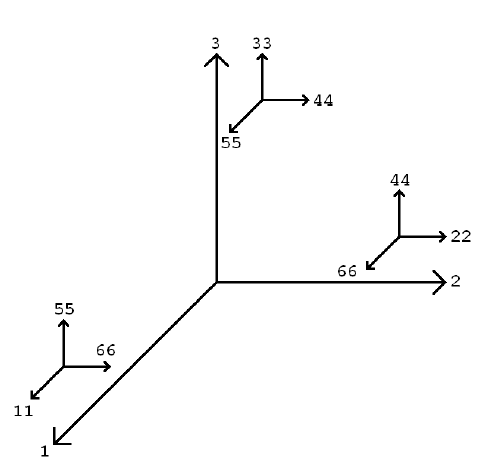
\includegraphics[width=0.5\textwidth]{png/speeds.png}}
\caption{Скорости распространения продольной и двух поперечных волн для каждой квазиодномерной волны.}
\label{pic:speeds-waves}
\end{figure}

\subsubsection{Трансверсальньно изотропное тело}
	
	Следующий тип анизотропии предполагает наличие во всех точках параллельных плоскостей упругой симметрии\cite{lehnitsky}.
	Иначе говоря, в каждой точке есть плоскость все направления в которой эквивалентны, а также есть выделенное направление, нормальное к плоскости.
	
	Примем за выделенное направление множество векторов коллинеарных оси $Z$, тогда плоскости изотропии будут параллельны плоскости $XY$.
	Матрица упругих постоянных имеет в этом случае всего пять независимых компонент:
\begin{align}
\label{vert_trans_tensor}
\left( \begin{array}{cccccccccccc}
c_{11} & c_{12} & c_{13} & 0 & 0 & 0 \\ 
c_{12} & c_{11} & c_{13} & 0 & 0 & 0 \\ 
c_{13} & c_{13} & c_{33} & 0 & 0 & 0 \\ 
0 & 0 & 0 & c_{44} & 0 & 0 \\ 
0 & 0 & 0 & 0 & c_{44} & 0 \\ 
0 & 0 & 0 & 0 & 0 & c_{66}
\end{array} \right){}
\end{align}
	где компоненты $c_{11}$, $c_{12}$, $c_{66}$ связаны соотношением:
\begin{equation}
	c_{66} = \frac{c_{11} - c_{12}}{2}.
\end{equation}

	Тензор упругих постоянных в этом случае похож на его аналог для орторомбической анизотропии, но тут он имеет меньшее количество независимых компонент.
	Это значит, что матрицы $\mathbf{A}_x$, $\mathbf{A}_y$, $\mathbf{A}_z$, а значит и собственные значения и собственные строки, имеют вид \eqref{orthorombic_mat1}-\eqref{orthorombic_mat3} с той лишь разницей, что некоторые компоненты зависимы и выражаются через другие.
	
	Данный вид анизотропии типичен для гексагональных решёток, а также для матрицы, аримированной однонаправленными волокнами -- основы ПКМ.
	
\subsection{Преобразование тензора упругих постоянных при повороте базиса}
	
	Многослойные ПКМ состоят из одинаковых слоёв, по-разному ориентированных вокруг оси укладки композита.
	Для расчёта конструкций необходимо найти вид тензора упругих постоянных в произвольно ориентированном базисе \cite{favorskaya}.
	
	Пусть $\theta_{x}$, $\theta_{y}$, $\theta_{z}$ -- углы поворота вокруг осей $x$, $y$, $z$ соответственно. 
	Чтобы перейти от старого базиса к новому нужно произвести последовательно эти повороты.
	Матрицы поворота будут иметь вид:
\begin{align}
\label{rotation_mat1}
\mathbf{G}_x =
\left( \begin{array}{cccccccccccc}
1 & 0 & 0 \\ 
0 & \cos \theta_{x} & -\sin \theta_{x} \\ 
0 & \sin \theta_{x} & \cos \theta_{x}
\end{array} \right),
\end{align} 
\begin{align}
\label{rotation_mat2}
\mathbf{G}_y =
\left( \begin{array}{cccccccccccc}
\cos \theta_{y} & 0 & \sin \theta_{y} \\
0 & 1 & 0 \\ 
-\sin \theta_{y} & 0 & \cos \theta_{y} 
\end{array} \right),
\end{align}
\begin{align}
\label{rotation_mat3}
\mathbf{G}_z =
\left( \begin{array}{cccccccccccc}
\cos \theta_{z} & -\sin \theta_{z} & 0 \\ 
\sin \theta_{z} & \cos \theta_{z} & 0 \\  
0 & 0 & 1  
\end{array} \right).
\end{align}
	
	Итоговая матрица преобразования базиса $\mathbf{G} = \mathbf{G}_{x}\mathbf{G}_{y}\mathbf{G}_{z}$ имеет вид:
\begin{align}
\label{rotation_mat}
\left( \begin{array}{cccccccccccc}
\cos \theta_{y} \cos \theta_{z} & \cos \theta_{z} \sin \theta_{x} \sin \theta_{y} - \sin \theta_{z} \cos \theta_{x} & \cos \theta_{x} \sin \theta_{y} \cos \theta_{z} + \sin \theta_{x} \sin \theta_{z} \\ 
\cos \theta_{y} \sin \theta_{z} & \sin \theta_{z} \sin \theta_{x} \sin \theta_{y} + \cos \theta_{z} \cos \theta_{x} & \cos \theta_{x} \sin \theta_{y} \sin \theta_{z} - \sin \theta_{x} \cos \theta_{z} \\ 
- \sin \theta_{y} & \sin \theta_{x} \cos \theta_{y} & \cos \theta_{x} \cos \theta_{y}
\end{array} \right)
\end{align}


	В итоге, тензор упругих постоянных $C_{ijkl}$, обсуждаемый в пункте 2.1, при поворотах системы координат будет преобразовываться по закону:
\begin{align}
	C_{mnpq} = \sum_{i,\;j,\;k,\;l = 1}^{3} g_{mi}\;g_{nj}\;g_{pk}\;g_{ql}\;C_{ijkl},
\end{align}
	где $g_{ij}$ -- тензор поворота, соответствующий матрице $\mathbf{G}$.
